\documentclass[aspectratio=169,10pt]{beamer}
\usepackage{issa}  % place issa.sty in the same folder
\usepackage{colortbl}
\definecolor{AccentCol}{HTML}{3949AB}
\renewcommand{\lecnum}{8}
\title{AI \& Machine Learning in Warfare}

\newcommand{\hc}[4]{%
 \pgfmathsetmacro{\pct}{int(round(100*#3))}%
 \fill[AccentCol!\pct!white] (#1,#2) rectangle ++(1,1);
 \draw[white,line width=0.8pt] (#1,#2) rectangle ++(1,1);
 \node[font=\scriptsize,text=\ifdim #3pt>0.5pt white\else ISSAdark\fi] at (#1+0.5,#2+0.5) {#4};}
\tikzset{tok/.style={nd,font=\scriptsize,minimum width=1.0cm,minimum height=0.55cm},
 blk/.style={draw=ISSAdark!70,rounded corners=2pt,minimum width=2.6cm,minimum height=0.55cm,font=\fontsize{7.5}{8.5}\selectfont,align=center,line width=0.5pt}}
% illustrative 7x7 head map for "recon drone spotted enemy armour near ford"
\newcommand{\headmap}[2]{%
\begin{tikzpicture}[scale=0.42]
\foreach \c [count=\j from 0] in {recon,drone,spotted,enemy,armour,near,ford}{\node[font=\tiny,anchor=south west,rotate=45] at (\j+0.3,7.05) {\c};}
\foreach \r [count=\i from 0] in {recon,drone,spotted,enemy,armour,near,ford}{\node[font=\tiny,anchor=east] at (-0.05,6.5-\i) {\r};}
\foreach \v [count=\k from 0] in {#1}{\pgfmathtruncatemacro{\rr}{\k/7}\pgfmathtruncatemacro{\cc}{mod(\k,7)}\hc{\cc}{6-\rr}{\v}{}}
\node[lab,anchor=north,font=\scriptsize] at (3.5,-0.1) {#2};
\end{tikzpicture}}

\begin{document}
\titleslide{8}{Transformers, Intuitively}{An analogy-first walk-through: meaning as coordinates, words that change with context, attention as a radio net, and how the encoder and decoder share the work}


%====================================================================
\sect{1. Overview}
\begin{frame}{Learning Objectives \& Session Structure}
\begin{columns}[T]
\column{0.55\textwidth}
\begin{cbox}{By the end of this lecture you will be able to}
\begin{te}
\item Explain what a language model does, and how it writes one token at a time
\item Describe embeddings as coordinates on a ``meaning map''
\item Explain why a fixed vector per word fails, and what a contextual vector is
\item Describe the jobs of the encoder and the decoder
\item Explain attention using queries, keys and values --- and compute one by hand
\item Explain multi-head attention, residual connections, normalisation and the feed-forward layer
\item Explain cross-attention in an encoder--decoder model
\end{te}
\end{cbox}
\column{0.42\textwidth}
\begin{cbox}[ISSAnavy]{Session Structure (45 min)}
\begin{tl}
\item \textbf{5 min} --- Opening Q\&A: CNNs (L7)
\item \textbf{10 min} --- Language models; meaning as numbers; the ``battery'' problem
\item \textbf{6 min} --- Encoder, decoder, tokens, positions
\item \textbf{14 min} --- Attention, multi-head, the full block, the decoder
\item \textbf{10 min} --- Auto-quiz (15 questions)
\end{tl}
\end{cbox}
\begin{ibox}\textbf{How this lecture fits:} it builds intuition. Lecture~9, \emph{Transformers \& Attention}, gives the full mathematics and the Vaswani et al.\ architecture block by block.\end{ibox}
\end{columns}
\end{frame}

\begin{frame}{What a Language Model Actually Does}
\begin{columns}[T]
\column{0.52\textwidth}
\figc{3.4cm}{%
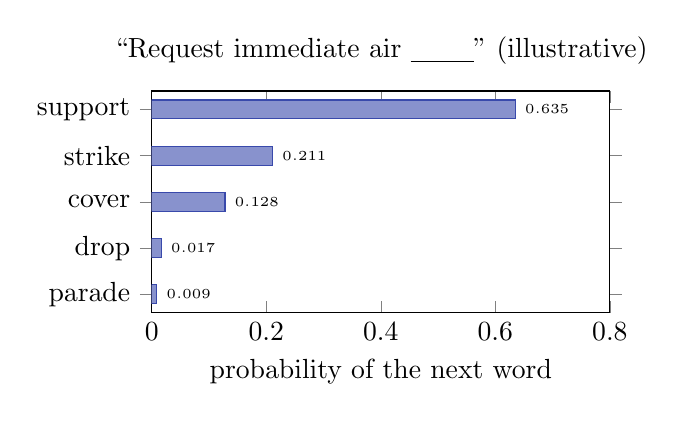
\begin{tikzpicture}
\begin{axis}[width=7.4cm,height=4.4cm,xbar,bar width=0.24cm,xmin=0,xmax=0.8,ytick=data,yticklabels={support,strike,cover,drop,parade},y dir=reverse,xlabel={probability of the next word},title={``Request immediate air \underline{\hspace{0.8cm}}'' (illustrative)},nodes near coords,nodes near coords style={font=\fontsize{5.5}{6.5}\selectfont,/pgf/number format/.cd,fixed,precision=3}]
\addplot[fill=AccentCol!60,draw=AccentCol] coordinates{(0.635,1)(0.211,2)(0.128,3)(0.017,4)(0.009,5)};
\end{axis}
\end{tikzpicture}}
\scriptsize Scores $(3.1,\,2.0,\,1.5,\,-0.5,\,-1.2)$ turned into probabilities by softmax.
\begin{cbox}{One job: predict the next token}\scriptsize Given the words so far, a language model outputs a probability for every token in its vocabulary. ``Parade'' is possible but unlikely; ``support'' fits what the model has seen in thousands of similar sentences.\end{cbox}
\column{0.45\textwidth}
\subhead{Writing a whole answer = repeating the job}
\figc{3.0cm}{%
\begin{tikzpicture}[node distance=0.25cm]
\node[nd,font=\scriptsize,text width=4.2cm] (s1) {Request immediate air \textbf{\textcolor{AccentCol}{support}}};
\node[nd,font=\scriptsize,text width=4.2cm,below=of s1] (s2) {Request immediate air support \textbf{\textcolor{AccentCol}{at}}};
\node[nd,font=\scriptsize,text width=4.2cm,below=of s2] (s3) {Request immediate air support at \textbf{\textcolor{AccentCol}{grid}}};
\node[lab,below=0.1cm of s3] {\dots each new word is appended and fed back in};
\draw[arrA] (s1.east)to[bend left=40](s2.east); \draw[arrA] (s2.east)to[bend left=40](s3.east);
\end{tikzpicture}}
\begin{rbox}\scriptsize A chat assistant's long, fluent reply is this loop run hundreds of times. ``Large'' language models do the same job with billions of learned parameters and vast training text.\end{rbox}
\end{columns}
\end{frame}

\begin{frame}{The Journey Through This Lecture}
\figc{3.2cm}{%
\begin{tikzpicture}[node distance=0.35cm]
\node[ndG] (a) {text\\``radio battery\\died''};
\node[ndA,right=of a] (b) {\textbf{tokens}\\pieces of\\words};
\node[ndA,right=of b] (c) {\textbf{embeddings}\\coordinates\\on a map};
\node[ndA,right=of c] (d) {\textbf{+ position}\\word order};
\node[ndC,right=of d] (e) {\textbf{attention}\\words update\\each other};
\node[ndA,right=of e] (f) {\textbf{feed-forward}\\each word\\refined};
\node[ndN,right=of f] (g) {\textbf{output}\\next word,\\summary, label};
\draw[arr] (a)--(b); \draw[arr] (b)--(c); \draw[arr] (c)--(d); \draw[arr] (d)--(e); \draw[arr] (e)--(f); \draw[arr] (f)--(g);
\draw[arrA,rounded corners] (f.south)--++(0,-0.45)-|node[lab,pos=0.25,below]{one ``transformer block'' --- stacked many times}(e.south);
\end{tikzpicture}}
\vspace{4pt}
\begin{columns}[T]
\column{0.32\textwidth}
\begin{cbox}{Running example}\scriptsize The word \textbf{battery}: an \emph{artillery} battery or a \emph{radio} battery? We will watch a transformer work it out from context.\end{cbox}
\column{0.32\textwidth}
\begin{cbox}{Analogies used}\scriptsize Grid references (embeddings), a radio net (attention), a sensor suite (multi-head), margin notes (residuals).\end{cbox}
\column{0.32\textwidth}
\begin{wbox}\scriptsize Analogies build intuition but are not the mechanism. Each slide also shows what is \emph{actually} computed.\end{wbox}
\end{columns}
\end{frame}

%====================================================================
\sect{2. Meaning as Numbers}
\begin{frame}{Why a Simple ID Number Is Not Enough}
\begin{columns}[T]
\column{0.48\textwidth}
\begin{cbox}{Computers need numbers}\scriptsize A model cannot read letters. The simplest idea is to number every word in a dictionary:
\begin{center}\renewcommand{\arraystretch}{1.1}
\begin{tabular}{lr}
\toprule\textbf{word}&\textbf{ID}\\\midrule
howitzer&4\,118\\hospital&4\,119\\howl&4\,120\\\bottomrule
\end{tabular}\end{center}
\end{cbox}
\begin{wbox}\scriptsize IDs follow spelling, not meaning: \emph{howitzer} sits next to \emph{hospital}, and nothing in ``4\,118'' says it is a weapon. Arithmetic on IDs is meaningless.\end{wbox}
\column{0.49\textwidth}
\begin{cbox}{Better: give each word a position on a map}\scriptsize A military grid reference places a location by several coordinates; nearby references are nearby places. An \textbf{embedding} places a word by a list of numbers; nearby lists are words with similar meaning.\end{cbox}
\figc{2.6cm}{%
\begin{tikzpicture}[scale=0.55]
\draw[step=1,ISSAgrey!35] (0,0) grid (8,4);
\foreach \x/\y/\w/\c in {1.2/3.1/howitzer/ISSAred,2.1/2.4/mortar/ISSAred,1.6/1.8/artillery/ISSAred,6.1/3.0/hospital/ISSAgrn,6.9/2.2/clinic/ISSAgrn,5.6/1.5/medic/ISSAgrn,3.9/0.6/howl/ISSAblue}{\fill[\c] (\x,\y) circle (0.12); \node[font=\tiny,anchor=west] at (\x+0.1,\y) {\w};}
\node[lab,font=\tiny] at (4,-0.45) {a 2-D slice of a meaning map (illustrative)};
\end{tikzpicture}}
\end{columns}
\end{frame}

\begin{frame}{Directions on the Meaning Map Carry Meaning}
\begin{columns}[T]
\column{0.52\textwidth}
\figc{5.0cm}{%
\begin{tikzpicture}
\begin{axis}[width=7.2cm,height=5.8cm,xmin=-1.6,xmax=2.6,ymin=-0.2,ymax=1.9,grid=major,grid style={ISSAgrey!20},xlabel={action type (illustrative)},ylabel={present $\longrightarrow$ past tense},title={Toy embedding space: verbs and their past tense},xticklabels={},yticklabels={}]
\addplot[only marks,mark=*,mark size=1.8pt,ISSAblue] coordinates{(1.0,0.2)(-1.0,0.25)(2.0,0.1)};
\addplot[only marks,mark=*,mark size=1.8pt,ISSAred] coordinates{(1.1,1.4)(-0.95,1.5)(2.1,1.3)};
\draw[-{Stealth[length=5pt]},AccentCol,line width=1.2pt] (axis cs:1.0,0.28)--(axis cs:1.1,1.32);
\draw[-{Stealth[length=5pt]},AccentCol,line width=1.2pt] (axis cs:-1.0,0.33)--(axis cs:-0.95,1.42);
\draw[-{Stealth[length=5pt]},AccentCol,line width=1.2pt] (axis cs:2.0,0.18)--(axis cs:2.1,1.22);
\node[font=\scriptsize,anchor=north] at (axis cs:1.0,0.15) {advance};
\node[font=\scriptsize,anchor=south] at (axis cs:1.1,1.45) {advanced};
\node[font=\scriptsize,anchor=north] at (axis cs:-1.0,0.2) {retreat};
\node[font=\scriptsize,anchor=south] at (axis cs:-0.95,1.55) {retreated};
\node[font=\scriptsize,anchor=north] at (axis cs:2.0,0.05) {attack};
\node[font=\scriptsize,anchor=south] at (axis cs:2.1,1.35) {attacked};
\end{axis}
\end{tikzpicture}}
\column{0.45\textwidth}
\begin{cbox}{A ``past-tense'' direction}\scriptsize In a well-trained space, the step from \emph{advance} to \emph{advanced} points roughly the same way as \emph{retreat}$\to$\emph{retreated} and \emph{attack}$\to$\emph{attacked}. Grammar has become geometry.\end{cbox}
\begin{fbx}{Vector arithmetic (toy numbers)}
$\overrightarrow{\text{retreat}}-\overrightarrow{\text{advance}}+\overrightarrow{\text{advanced}}$\\
$=(-1.0,0.25)-(1.0,0.2)+(1.1,1.4)=(-0.9,\,1.45)$\\[2pt]
nearest word: \textbf{retreated} $(-0.95,1.5)$
\end{fbx}
\begin{ibox}\scriptsize Other directions found in real embeddings: singular$\to$plural, country$\to$capital, unit$\to$parent formation. Lecture~9 works the classic male$\to$female example in full.\end{ibox}
\end{columns}
\end{frame}

\begin{frame}{Where Embeddings Come From}
\begin{columns}[T]
\column{0.50\textwidth}
\begin{cbox}{Nobody writes them by hand}\scriptsize The numbers start random. The model reads enormous amounts of text, repeatedly tries to predict missing or next words, and backpropagation nudges every word's vector until predictions improve. Words used in similar company end up close together.\end{cbox}
\begin{wbox}\scriptsize\textbf{The dimensions have no names.} Our toy axes (``action type'', ``tense'') are labelled for teaching; in a real model meaning is spread across hundreds or thousands of unlabelled numbers.\end{wbox}
\column{0.47\textwidth}
\centering\scriptsize\renewcommand{\arraystretch}{1.25}
\begin{tabular}{lr}
\toprule
\textbf{Model}&\textbf{numbers per token}\\\midrule
word2vec (2013)&300\\
BERT-base (2018)&768\\
GPT-2 small (2019)&768\\
GPT-3 (2020)&12\,288\\\bottomrule
\end{tabular}
\vspace{4pt}
\raggedright
\begin{rbox}\scriptsize We can draw two or three dimensions; the mathematics works the same in 12\,288. More dimensions leave room for finer shades of meaning.\end{rbox}
\begin{ibox}\scriptsize word2vec and GloVe produce \textbf{static} embeddings: one fixed vector per word. That turns out not to be enough \dots\end{ibox}
\end{columns}
\end{frame}

%====================================================================
\sect{3. Static vs Contextual}
\begin{frame}{The ``Battery'' Problem: One Word, Several Meanings}
\begin{columns}[T]
\column{0.50\textwidth}
\begin{cbox}{Same spelling, different meaning}\scriptsize
\begin{tl}
\item ``The artillery \textbf{battery} fired at dawn.'' \ --- a unit of guns
\item ``The radio \textbf{battery} died at dawn.'' \ --- a power cell
\item ``The suspect was charged with \textbf{battery}.'' \ --- an offence
\end{tl}
\end{cbox}
\begin{wbox}\scriptsize A \textbf{static} embedding gives ``battery'' one point on the map --- somewhere between guns and power cells. The model then has to guess which meaning is intended, and the next-word predictions blur.\end{wbox}
\column{0.47\textwidth}
\begin{cbox}{What the next word depends on}\scriptsize
\centering\renewcommand{\arraystretch}{1.15}
\begin{tabular}{ll}
\toprule\textbf{context so far}&\textbf{likely next words}\\\midrule
the artillery battery \dots&fired, displaced, commander\\
the radio battery \dots&died, charged, pack\\\bottomrule
\end{tabular}
\end{cbox}
\begin{rbox}\scriptsize\textbf{Goal:} a \textbf{contextual} embedding --- a vector for ``battery'' that has been \emph{pulled} by its neighbours towards the right meaning, for this sentence only.\end{rbox}
\begin{ibox}\scriptsize Producing contextual embeddings is the central job of every transformer layer.\end{ibox}
\end{columns}
\end{frame}

\begin{frame}{Running Example: Context Pulls ``Battery'' Two Different Ways}
\begin{columns}[T]
\column{0.50\textwidth}
\figc{5.2cm}{%
\begin{tikzpicture}
\begin{axis}[width=7cm,height=6cm,xmin=0,xmax=3.8,ymin=0,ymax=3.8,grid=major,grid style={ISSAgrey!20},xlabel={``military'' direction (toy)},ylabel={``electrical'' direction (toy)},title={2-D toy meaning map}]
\addplot[only marks,mark=*,mark size=1.8pt,ISSAred] coordinates{(3,0.2)(2.4,0.4)};
\addplot[only marks,mark=*,mark size=1.8pt,ISSAgrn] coordinates{(0.2,3)(0.4,2.2)};
\addplot[only marks,mark=square*,mark size=2.4pt,ISSAgrey] coordinates{(1,1)};
\node[font=\scriptsize,anchor=west] at (axis cs:3.0,0.2) {artillery};
\node[font=\scriptsize,anchor=north] at (axis cs:2.4,0.35) {fired};
\node[font=\scriptsize,anchor=west] at (axis cs:0.25,3.05) {radio};
\node[font=\scriptsize,anchor=west] at (axis cs:0.45,2.2) {died};
\node[font=\scriptsize,anchor=north] at (axis cs:1.0,0.9) {battery (static)};
\draw[-{Stealth[length=5pt]},AccentCol,line width=1.3pt] (axis cs:1.08,1.02)--(axis cs:3.33,1.41);
\draw[-{Stealth[length=5pt]},AccentCol,line width=1.3pt] (axis cs:1.02,1.08)--(axis cs:1.41,3.27);
\addplot[only marks,mark=diamond*,mark size=2.8pt,AccentCol] coordinates{(3.40,1.43)(1.43,3.34)};
\node[font=\fontsize{5.5}{6.5}\selectfont,text=AccentCol,anchor=south] at (axis cs:3.2,1.5) {battery in A};
\node[font=\fontsize{5.5}{6.5}\selectfont,text=AccentCol,anchor=west] at (axis cs:1.5,3.4) {battery in B};
\end{axis}
\end{tikzpicture}}
\column{0.47\textwidth}
\begin{cbox}{Two sentences}\scriptsize
\textbf{A}: ``artillery \textbf{battery} fired'' \qquad \textbf{B}: ``radio \textbf{battery} died''\\
Toy vectors: artillery $(3,0.2)$, fired $(2.4,0.4)$, radio $(0.2,3)$, died $(0.4,2.2)$, battery $(1,1)$
\end{cbox}
\begin{cbox}{Result of one attention step (next slides)}\scriptsize
\renewcommand{\arraystretch}{1.15}\centering
\begin{tabular}{lcc}
\toprule&\textbf{sentence A}&\textbf{sentence B}\\\midrule
attention output $z$&$(2.40,\,0.43)$&$(0.43,\,2.34)$\\
battery $+\,z$&$(3.40,\,1.43)$&$(1.43,\,3.34)$\\\bottomrule
\end{tabular}
\end{cbox}
\begin{rbox}\scriptsize The \emph{same} starting vector for ``battery'' moves towards the guns in A and towards the power cells in B. That moved vector is its \textbf{contextual embedding}.\end{rbox}
\end{columns}
\end{frame}

\begin{frame}{Context Can Come From Far Away}
\centering
\begin{tikzpicture}[x=1.2cm]
\foreach \w [count=\i] in {The,pilot,who,trained,the,new,cadets,for,three,years,finally,retired}{\node[tok,minimum width=1.0cm,font=\fontsize{6.5}{7.5}\selectfont] (t\i) at (\i,0) {\w};}
\node[tok,fill=AccentCol!25,draw=AccentCol,minimum width=1.0cm,font=\fontsize{6.5}{7.5}\selectfont] at (12,0) {retired};
\draw[-{Stealth[length=5pt]},AccentCol,line width=2.4pt] (t12.north) to[bend right=18] node[lab,above,font=\scriptsize\bfseries,text=AccentCol,fill=ISSAvlight,inner sep=1pt]{strong} (t2.north);
\draw[-{Stealth[length=5pt]},AccentCol!35,line width=0.7pt] (t12.south) to[bend left=25] node[lab,below,font=\scriptsize]{weak} (t7.south);
\end{tikzpicture}
\vspace{2pt}
\raggedright
\begin{columns}[T]
\column{0.32\textwidth}
\begin{cbox}{Who retired?}\scriptsize The pilot --- nine words earlier --- not the nearer ``cadets'' or ``years''. Looking only at the last few words gets this wrong.\end{cbox}
\column{0.32\textwidth}
\begin{cbox}{Clues can be paragraphs away}\scriptsize ``\dots trained for months on the new 155\,mm guns \dots [three sentences later] \dots at dawn the \textbf{battery} \underline{\hspace{0.5cm}}'' --- the deciding clue is far back.\end{cbox}
\column{0.32\textwidth}
\begin{rbox}\scriptsize\textbf{Attention looks at every word, however distant}, and weighs its relevance. Distance alone does not decide.\end{rbox}
\end{columns}
\begin{ibox}\scriptsize Older recurrent networks passed information word by word, so clues faded over long distances. Removing that bottleneck is why transformers handle long reports well.\end{ibox}
\end{frame}

%====================================================================
\sect{4. Encoder \& Decoder}
\begin{frame}{Two Halves: The Encoder Reads, the Decoder Writes}
\figc{3.3cm}{%
\begin{tikzpicture}[node distance=0.45cm]
\node[ndG,text width=3.2cm] (in) {``Two enemy tanks moving north near the bridge at 0600''};
\node[ndC,right=of in,minimum width=2.4cm,minimum height=1.2cm] (enc) {\textbf{ENCODER}\\understands the\\whole report};
\node[ndY,right=of enc,text width=2.4cm] (ctx) {contextual vector\\for every input word};
\node[ndC,right=of ctx,minimum width=2.4cm,minimum height=1.2cm] (dec) {\textbf{DECODER}\\writes the output\\one token at a time};
\node[ndN,right=of dec,text width=2.6cm] (out) {SIZE: 2\\ACTIVITY: moving north\\LOCATION: bridge\\TIME: 0600 \dots};
\draw[arr] (in)--(enc); \draw[arr] (enc)--(ctx); \draw[arr] (ctx)--(dec); \draw[arr] (dec)--(out);
\draw[arrA,rounded corners] (out.south)--++(0,-0.45)-|node[lab,pos=0.25,below]{each token written is fed back to the decoder}(dec.south);
\end{tikzpicture}}
\begin{columns}[T]
\column{0.32\textwidth}
\begin{cbox}{Encoder}\scriptsize Reads the whole input at once and produces a contextual embedding for each token.\end{cbox}
\column{0.32\textwidth}
\begin{cbox}{Decoder}\scriptsize Starts from a special \emph{start} token; at each step uses (1) the encoder's vectors and (2) everything it has written so far.\end{cbox}
\column{0.32\textwidth}
\begin{cbox}{Same pattern, many tasks}\scriptsize Free text $\to$ structured report (shown), translation, summarisation, question answering.\end{cbox}
\end{columns}
\end{frame}

\begin{frame}{Training vs Inference: Learning From Text That Labels Itself}
\begin{columns}[T]
\column{0.52\textwidth}
\subhead{One sentence becomes many training examples}
\centering\scriptsize\renewcommand{\arraystretch}{1.15}
\begin{tabular}{ll}
\toprule\textbf{input $x$ (words so far)}&\textbf{target $y$}\\\midrule
Request&immediate\\
Request immediate&air\\
Request immediate air&support\\
Request immediate air support&for\\
Request immediate air support for&the\\
Request immediate air support for the&platoon\\\bottomrule
\end{tabular}
\raggedright\vspace{3pt}
\begin{ibox}\scriptsize\textbf{Self-supervised:} no human labelling --- the next word in real text \emph{is} the label. Any manual, report or book becomes training data.\end{ibox}
\column{0.45\textwidth}
\begin{cbox}{Training}\scriptsize The untrained model guesses (say ``drop'' instead of ``support''); the error is measured with cross-entropy and backpropagated. Across billions of examples this sets the embeddings, the attention matrices $W^Q,W^K,W^V$ and every other weight.\end{cbox}
\begin{cbox}[ISSAnavy]{Inference}\scriptsize The trained model is used on new text with its weights \emph{frozen}. Everything later in this lecture describes what happens at inference.\end{cbox}
\begin{rbox}\scriptsize Like a cadet: years of drills (training), then decisions in the field using what was learned (inference).\end{rbox}
\end{columns}
\end{frame}

\begin{frame}{BERT, GPT and the Original Design}
\begin{columns}[T]
\column{0.45\textwidth}
\figc{5.2cm}{%
\begin{tikzpicture}[node distance=0.3cm]
\node[ndC,minimum width=1.6cm,minimum height=1.0cm] (e1) {encoder}; \node[ndC,right=of e1,minimum width=1.6cm,minimum height=1.0cm] (d1) {decoder}; \draw[arr] (e1)--(d1);
\node[lab,below=0.1cm of e1,xshift=0.95cm,font=\scriptsize] {original Transformer, T5};
\node[ndC,below=0.9cm of e1,minimum width=1.6cm,minimum height=1.0cm] (e2) {encoder}; \node[nd,right=of e2,minimum width=1.6cm,minimum height=1.0cm,draw=ISSAgrey!40,text=ISSAgrey!60,dashed] (d2) {---};
\node[lab,below=0.1cm of e2,xshift=0.95cm,font=\scriptsize] {BERT (encoder only)};
\node[nd,below=0.9cm of e2,minimum width=1.6cm,minimum height=1.0cm,draw=ISSAgrey!40,text=ISSAgrey!60,dashed] (e3) {---}; \node[ndC,right=of e3,minimum width=1.6cm,minimum height=1.0cm] (d3) {decoder};
\node[lab,below=0.1cm of e3,xshift=0.95cm,font=\scriptsize] {GPT family (decoder only)};
\end{tikzpicture}}
\column{0.47\textwidth}
\centering\scriptsize\renewcommand{\arraystretch}{1.25}
\begin{tabular}{lrr}
\toprule&\textbf{BERT-base}&\textbf{GPT-3}\\\midrule
part used&encoder&decoder\\
numbers per token&768&12\,288\\
layers (blocks)&12&96\\
attention heads&12&96\\
vocabulary&30\,522&$\approx$50\,000\\
best at&understanding&generating\\\bottomrule
\end{tabular}
\raggedright\vspace{3pt}
\begin{ibox}\scriptsize ``Transformer'' is the general design; BERT and GPT are particular models built from it. A GPT-style decoder still builds contextual embeddings --- it simply uses only the words to its left.\end{ibox}
\end{columns}
\end{frame}

%====================================================================
\sect{5. Tokens \& Positions}
\begin{frame}{Inside the Encoder, Step 1: Tokens and Token IDs}
\figc{2.6cm}{%
\begin{tikzpicture}[node distance=0.2cm]
\node[ndG,minimum width=6cm] (s) {``Reconnaissance team located the battery''};
\node[tok,below left=0.7cm and 2.6cm of s.south,fill=ISSAyell] (a) {[CLS]};
\node[tok,right=of a] (b) {recon};
\node[tok,right=of b] (c) {\#\#naissance};
\node[tok,right=of c] (d) {team};
\node[tok,right=of d] (e) {located};
\node[tok,right=of e] (f) {the};
\node[tok,right=of f] (g) {battery};
\node[tok,right=of g,fill=ISSAyell] (h) {[SEP]};
\foreach \n/\id in {a/101,b/28667,c/15055,d/2136,e/2284,f/1996,g/6046,h/102}{\node[ndY,below=0.4cm of \n,font=\scriptsize] (i\n) {\id}; \draw[arr] (\n)--(i\n);}
\draw[arr] (s.south)--(d.north);
\end{tikzpicture}}
\begin{columns}[T]
\column{0.32\textwidth}
\begin{cbox}{Tokens, not words}\scriptsize Common words are one token; long or rare words split into pieces (``\#\#'' marks a continuation in BERT's tokenizer). Treating tokens as words is fine for intuition.\end{cbox}
\column{0.32\textwidth}
\begin{cbox}{Special tokens}\scriptsize BERT adds [CLS] at the start (a summary slot, used for classification) and [SEP] to mark the end of a sentence or the boundary between two.\end{cbox}
\column{0.32\textwidth}
\begin{ibox}\scriptsize Each token has an ID: its row number in the vocabulary (30\,522 entries for BERT). [CLS]~$=101$ and [SEP]~$=102$ in BERT; the other IDs here are illustrative.\end{ibox}
\end{columns}
\end{frame}

\begin{frame}{Step 2: Look Up Each Token's Vector}
\begin{columns}[T]
\column{0.55\textwidth}
\figc{4.0cm}{%
\begin{tikzpicture}[scale=0.5]
\node[font=\scriptsize] at (3.5,8.6) {embedding matrix ($V$ rows $\times\ d$ columns)};
\foreach \r in {0,...,7}{\foreach \c in {0,...,6}{\pgfmathsetmacro{\sh}{int(10+mod(\r*37+\c*53,40))}\fill[AccentCol!\sh!white] (\c,\r) rectangle ++(1,1);}}
\draw[ISSAgrey] (0,0) grid (7,8);
\fill[ISSAamb!50] (0,4) rectangle (7,5); \draw[ISSAamb,line width=1.4pt] (0,4) rectangle (7,5);
\node[font=\scriptsize,anchor=east] at (-0.2,4.5) {row 6046};
\node[font=\scriptsize,anchor=east] at (-0.2,7.5) {row 0};
\node[font=\scriptsize,anchor=east] at (-0.2,0.5) {row 30\,521};
\draw[-{Stealth[length=4pt]},AccentCol,line width=1pt] (7.3,4.5)--(9.3,4.5);
\foreach \c in {0,...,6}{\fill[ISSAamb!50] (9.6+\c*0.9,4.05) rectangle ++(0.8,0.9);}
\node[font=\scriptsize,anchor=north] at (12.7,3.8) {static vector for ``battery''};
\node[font=\scriptsize,anchor=north] at (12.7,3.0) {(768 numbers in BERT)};
\end{tikzpicture}}
\column{0.42\textwidth}
\begin{cbox}{A lookup, not a calculation}\scriptsize The token ID is simply a row number. The model copies that row --- the token's \textbf{static embedding}. The whole table was learned during training.\end{cbox}
\begin{cbox}[ISSAnavy]{What training also learned}\scriptsize Besides this table, training fixed the attention matrices $W^Q$, $W^K$, $W^V$ and all the other weights we meet next. At inference none of them change.\end{cbox}
\begin{ibox}\scriptsize At this point ``battery'' has the \emph{same} vector in every sentence. The next steps make it context-aware.\end{ibox}
\end{columns}
\end{frame}

\begin{frame}{Step 3: Stamp Each Vector With Its Position}
\begin{columns}[T]
\column{0.50\textwidth}
\begin{cbox}{Order changes meaning}\scriptsize
``\textbf{Alpha} relieves \textbf{Bravo}'' \quad vs \quad ``\textbf{Bravo} relieves \textbf{Alpha}''\\
Same words, opposite orders --- and opposite consequences for who stays in the line.
\end{cbox}
\begin{wbox}\scriptsize A transformer processes all tokens \textbf{in parallel}, not one after another. Without extra information it would see these two sentences as the same bag of words.\end{wbox}
\begin{fbx}{Fix: add a position vector}
$\text{input}_t=\text{embedding}_t+\text{position}_t$
\end{fbx}
\column{0.47\textwidth}
\figc{2.6cm}{%
\begin{tikzpicture}[node distance=0.25cm]
\foreach \w/\x in {Alpha/0,relieves/2.2,Bravo/4.4}{\node[tok,minimum width=1.6cm] (w\w) at (\x,0) {\w};}
\foreach \w/\x/\p in {Alpha/0/1,relieves/2.2/2,Bravo/4.4/3}{\node[ndY,minimum width=1.6cm,font=\scriptsize] (p\w) at (\x,-1.0) {position \p}; \node[font=\small] at (\x,-0.5) {$+$};}
\foreach \w/\x in {Alpha/0,relieves/2.2,Bravo/4.4}{\node[ndA,minimum width=1.6cm,font=\scriptsize] at (\x,-2.0) {meaning + place}; \draw[arr] (p\w)--(\x,-1.72);}
\end{tikzpicture}}
\begin{cbox}{How the position vectors are made}\scriptsize The original paper used sine and cosine waves of many frequencies --- like reading a clock's second, minute and hour hands together --- so every position gets a unique, bounded code. Many later models learn the position vectors instead.\end{cbox}
\begin{ibox}\scriptsize The formula and a worked example are in Lecture~9.\end{ibox}
\end{columns}
\end{frame}

%====================================================================
\sect{6. Attention}
\begin{frame}{Step 4: Attention --- Which Words Should Update Which?}
\begin{columns}[T]
\column{0.52\textwidth}
\figc{3.6cm}{%
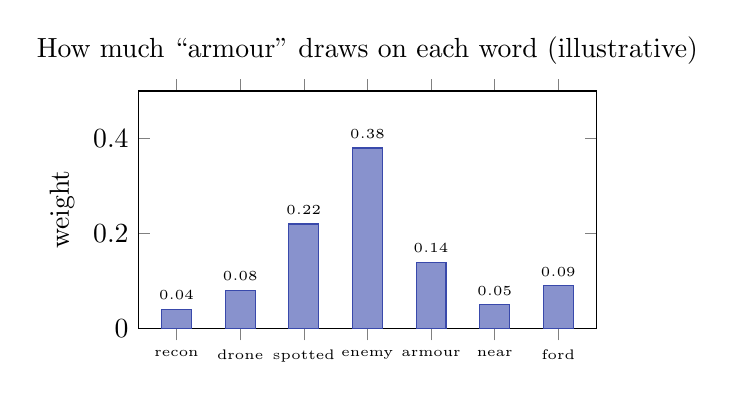
\begin{tikzpicture}
\begin{axis}[width=7.4cm,height=4.6cm,ybar,bar width=0.38cm,ymin=0,ymax=0.5,xtick=data,xticklabels={recon,drone,spotted,enemy,armour,near,ford},x tick label style={font=\fontsize{5.5}{6.5}\selectfont},ylabel={weight},title={How much ``armour'' draws on each word (illustrative)},nodes near coords,nodes near coords style={font=\fontsize{5}{6}\selectfont,/pgf/number format/.cd,fixed,precision=2}]
\addplot[fill=AccentCol!60,draw=AccentCol] coordinates{(1,0.04)(2,0.08)(3,0.22)(4,0.38)(5,0.14)(6,0.05)(7,0.09)};
\end{axis}
\end{tikzpicture}}
\scriptsize Sentence: ``recon drone spotted enemy armour near ford''
\column{0.45\textwidth}
\begin{cbox}{Reading the chart}\scriptsize ``enemy'' (0.38) tells us \emph{whose} armour; ``spotted'' (0.22) says what happened to it; ``armour'' itself (0.14) keeps its own meaning. ``recon'' adds little to the meaning of ``armour''. The weights sum to 1.\end{cbox}
\begin{rbox}\scriptsize Replace ``enemy'' with ``friendly'' and the contextual vector for ``armour'' changes a lot; replace ``near'' with ``by'' and it barely moves. High weight = big influence.\end{rbox}
\begin{ibox}\scriptsize Every word gets such a set of weights over every other word (and itself): an $n\times n$ table of attention weights.\end{ibox}
\end{columns}
\end{frame}

\begin{frame}{Query, Key, Value: The Radio-Net Analogy}
\figc{3.0cm}{%
\begin{tikzpicture}[node distance=0.35cm]
\node[ndC,minimum width=2.8cm,minimum height=1.1cm] (q) {\textbf{QUERY}\\``battery'' listens for:\\\emph{who tells me my role?}};
\node[nd,right=1.3cm of q,yshift=0.9cm,minimum width=2.6cm] (k1) {\textbf{Key} ``artillery'':\\\emph{I name a gun unit}};
\node[nd,right=1.3cm of q,minimum width=2.6cm] (k2) {\textbf{Key} ``the'':\\\emph{I am a determiner}};
\node[nd,right=1.3cm of q,yshift=-0.9cm,minimum width=2.6cm] (k3) {\textbf{Key} ``fired'':\\\emph{I am a weapon action}};
\node[ndG,right=0.3cm of k1,minimum width=2.2cm] (v1) {\textbf{Value:} gun-unit meaning};
\node[ndG,right=0.3cm of k2,minimum width=2.2cm] (v2) {\textbf{Value:} grammar info};
\node[ndG,right=0.3cm of k3,minimum width=2.2cm] (v3) {\textbf{Value:} firing meaning};
\draw[arrA,line width=1.8pt] (q.east)--node[lab,above,sloped]{loud}(k1.west);
\draw[arrA,line width=0.4pt] (q.east)--node[lab,above]{faint}(k2.west);
\draw[arrA,line width=1.3pt] (q.east)--node[lab,below,sloped]{loud}(k3.west);
\end{tikzpicture}}
\begin{columns}[T]
\column{0.32\textwidth}
\begin{cbox}{Query $q$}\scriptsize The call-sign a station is \textbf{listening for} --- what this word needs to know.\end{cbox}
\column{0.32\textwidth}
\begin{cbox}{Key $k$}\scriptsize The call-sign each station \textbf{transmits} --- what kind of information it offers. A good match $q\cdot k$ turns the volume up.\end{cbox}
\column{0.32\textwidth}
\begin{cbox}{Value $v$}\scriptsize The \textbf{message} itself. The listener hears every message, each at its own volume, and sums them.\end{cbox}
\end{columns}
\begin{ibox}\scriptsize The volume mixer always adds up to 100\% (softmax). The ``call-signs'' are not words like these in reality: they are learned vectors, and the model decides what to listen for.\end{ibox}
\end{frame}

\begin{frame}{Where $Q$, $K$ and $V$ Really Come From}
\begin{columns}[T]
\column{0.52\textwidth}
\figc{3.4cm}{%
\begin{tikzpicture}[node distance=0.4cm]
\node[ndA,minimum width=2.4cm,minimum height=0.8cm] (x) {embedding + position\\of ``battery''};
\node[ndN,right=1.2cm of x,yshift=0.95cm] (wq) {$\times W^{Q}$};
\node[ndN,right=1.2cm of x] (wk) {$\times W^{K}$};
\node[ndN,right=1.2cm of x,yshift=-0.95cm] (wv) {$\times W^{V}$};
\node[nd,right=0.45cm of wq,fill=AccentCol!25] (q) {query $q$};
\node[nd,right=0.45cm of wk,fill=ISSAamb!25,draw=ISSAamb] (k) {key $k$};
\node[nd,right=0.45cm of wv,fill=ISSAgrn!20,draw=ISSAgrn] (v) {value $v$};
\draw[arr] (x.east)--(wq.west); \draw[arr] (x.east)--(wk.west); \draw[arr] (x.east)--(wv.west);
\draw[arr] (wq)--(q); \draw[arr] (wk)--(k); \draw[arr] (wv)--(v);
\end{tikzpicture}}
\begin{fbx}{Three learned matrices, applied to every token}
$q=x\,W^{Q},\qquad k=x\,W^{K},\qquad v=x\,W^{V}$
\end{fbx}
\column{0.45\textwidth}
\begin{cbox}{What each matrix ``knows''}\scriptsize
\begin{tl}
\item $W^Q$: how to turn a token into a \emph{question}
\item $W^K$: how to turn a token into an \emph{advertisement}
\item $W^V$: how to turn a token into the \emph{content} it hands over
\end{tl}
All three are learned in (pre-)training and then fixed.
\end{cbox}
\begin{cbox}[ISSAnavy]{Sizes per head}\scriptsize BERT-base: $768\to64$ numbers; GPT-3: $12\,288\to128$. Each token's $q$, $k$ and $v$ are much shorter than its embedding.\end{cbox}
\begin{ibox}\scriptsize Every token is projected at the same time, so $Q$, $K$, $V$ are matrices with one row per token.\end{ibox}
\end{columns}
\end{frame}

\begin{frame}{The Recipe in Four Steps}
\figc{2.5cm}{%
\begin{tikzpicture}[node distance=0.5cm]
\node[ndA,text width=2.5cm] (s1) {\textbf{1. Match}\\$q\cdot k$ for every\\other token};
\node[ndA,right=of s1,text width=2.5cm] (s2) {\textbf{2. Scale}\\divide by $\sqrt{d_k}$};
\node[ndA,right=of s2,text width=2.5cm] (s3) {\textbf{3. Softmax}\\scores $\to$ weights\\summing to 1};
\node[ndC,right=of s3,text width=2.5cm] (s4) {\textbf{4. Blend}\\weighted sum of\\the values $v$};
\draw[arr] (s1)--(s2); \draw[arr] (s2)--(s3); \draw[arr] (s3)--(s4);
\end{tikzpicture}}
\begin{fbx}{All tokens at once}
$\text{Attention}(Q,K,V)=\text{softmax}\!\left(\dfrac{QK^{\mathsf T}}{\sqrt{d_k}}\right)V$
\end{fbx}
\begin{columns}[T]
\column{0.48\textwidth}
\begin{cbox}{Why the transpose $K^{\mathsf T}$?}\scriptsize For one query and one key, $q\cdot k$ is a single number. Stacking all keys as rows of $K$, the product $QK^{\mathsf T}$ computes every query--key match in one go: an $n\times n$ table.\end{cbox}
\column{0.48\textwidth}
\begin{cbox}{Why divide by $\sqrt{d_k}$?}\scriptsize Dot products grow with vector length. Without scaling, softmax would put nearly all weight on one word and learning would stall. GPT-3: $d_k=128$, divide by $11.3$.\end{cbox}
\end{columns}
\end{frame}

\begin{frame}{Worked Example: The Arithmetic Behind the ``Battery'' Picture}
\begin{columns}[T]
\column{0.55\textwidth}
\scriptsize Simplest case for hand arithmetic: $W^Q=W^K=W^V=I$ (identity), so $q=k=v=x$; $d_k=2$.
\vspace{2pt}

\subhead{Sentence A: ``artillery battery fired''}
\centering\scriptsize\renewcommand{\arraystretch}{1.15}
\begin{tabular}{lcccc}
\toprule\textbf{key}&$q_{\text{battery}}\cdot k$&$\div\sqrt2$&$e^{(\cdot)}$&\textbf{weight}\\\midrule
artillery $(3,0.2)$&3.2&2.263&9.609&\textbf{0.458}\\
battery $(1,1)$&2.0&1.414&4.113&0.196\\
fired $(2.4,0.4)$&2.8&1.980&7.242&0.345\\\midrule
&&&sum 20.965&1.000\\\bottomrule
\end{tabular}
\raggedright\vspace{3pt}
\scriptsize Blend: $z=0.458(3,0.2)+0.196(1,1)+0.345(2.4,0.4)=(\hl{2.40},\ \hl{0.43})$
\vspace{2pt}

Add to the original (residual): $(1,1)+(2.40,0.43)=(\hl{3.40},\ \hl{1.43})$ --- deep in ``military'' territory.
\column{0.42\textwidth}
\subhead{Sentence B: ``radio battery died''}
\scriptsize Scores $3.2,\,2.0,\,2.6$ $\to$ weights $0.480,\ 0.206,\ 0.314$
\[z=(0.43,\ 2.34),\qquad x+z=(1.43,\ 3.34)\]
\begin{rbox}\scriptsize Identical query, identical arithmetic --- different neighbours, so a different result. That is all a contextual embedding is.\end{rbox}
\begin{wbox}\scriptsize Real models use \emph{learned} $W^Q,W^K,W^V$, not the identity: the question a word asks can differ from what it advertises and what it hands over. Lecture~9 works that case.\end{wbox}
\end{columns}
\end{frame}

%====================================================================
\sect{7. Multi-Head}
\begin{frame}{Multi-Head Attention: A Sensor Suite, Not a Single Sensor}
\begin{columns}[T]
\column{0.52\textwidth}
\figc{3.8cm}{%
\begin{tikzpicture}[node distance=0.3cm]
\node[ndA,minimum width=1.8cm] (x) {token vectors};
\node[ndC,right=1.0cm of x,yshift=1.15cm] (h1) {head 1};
\node[ndC,right=1.0cm of x,yshift=0.38cm] (h2) {head 2};
\node[ndC,right=1.0cm of x,yshift=-0.38cm] (h3) {head 3};
\node[nd,right=1.0cm of x,yshift=-1.15cm] (h4) {head $h$};
\node[ndY,right=0.9cm of h2,yshift=-0.38cm] (c) {combine\\(concat $\times W^O$)};
\node[ndN,right=0.5cm of c] (o) {richer\\vectors};
\foreach \h in {h1,h2,h3,h4}{\draw[arr] (x.east)--(\h.west); \draw[arr] (\h.east)--(c.west);}
\draw[arr] (c)--(o);
\end{tikzpicture}}
\begin{cbox}{Each head has its own $W^Q,W^K,W^V$}\scriptsize So each asks a different question of the same sentence, in parallel. Their outputs are joined and mixed by one more matrix $W^O$.\end{cbox}
\column{0.45\textwidth}
\begin{cbox}{Analogy: a surveillance sensor suite}\scriptsize Radar, infrared and a camera watch the same scene. Each picks up what the others miss --- range, heat, shape --- and the fused picture beats any single sensor. Heads do the same for relationships between words.\end{cbox}
\begin{cbox}[ISSAnavy]{Real numbers}\scriptsize BERT-base: 12 heads $\times$ 64 = 768. \ GPT-3: 96 heads $\times$ 128 = 12\,288. The head size is chosen so the heads together match the embedding width.\end{cbox}
\begin{ibox}\scriptsize Nobody assigns roles to heads; specialisations emerge during training.\end{ibox}
\end{columns}
\end{frame}

\begin{frame}{What Different Heads Might Track (Illustrative)}
\begin{columns}[T]
\column{0.32\textwidth}
\centering\figc{3.3cm}{\headmap{0.3,0.6,0.05,0.05,0,0,0, 0.55,0.35,0.05,0.05,0,0,0, 0,0,0.3,0.1,0.5,0.05,0.05, 0,0,0.05,0.25,0.65,0.05,0, 0,0,0.05,0.6,0.3,0.05,0, 0,0,0,0,0.05,0.3,0.65, 0,0,0,0,0.05,0.35,0.6}{head A: modifiers}}
\begin{cbox}{Modifier head}\scriptsize ``enemy'' $\leftrightarrow$ ``armour'', ``recon'' $\leftrightarrow$ ``drone'': which words describe which.\end{cbox}
\column{0.32\textwidth}
\centering\figc{3.3cm}{\headmap{0.2,0.2,0.4,0.1,0.1,0,0, 0.05,0.2,0.6,0.05,0.1,0,0, 0.05,0.4,0.15,0.05,0.35,0,0, 0,0.1,0.6,0.2,0.1,0,0, 0,0.1,0.65,0.1,0.15,0,0, 0,0,0.3,0,0.3,0.2,0.2, 0,0,0.4,0,0.2,0.2,0.2}{head B: action}}
\begin{cbox}{Action head}\scriptsize ``spotted'' connects \emph{who} spotted (drone) with \emph{what} was spotted (armour).\end{cbox}
\column{0.32\textwidth}
\centering\figc{3.3cm}{\headmap{0.1,0.1,0.1,0.1,0.1,0.2,0.3, 0.05,0.1,0.15,0.05,0.15,0.2,0.3, 0,0.05,0.1,0,0.15,0.2,0.5, 0,0,0.1,0.1,0.2,0.2,0.4, 0,0,0.05,0.05,0.1,0.3,0.5, 0,0,0,0,0.2,0.2,0.6, 0,0,0.1,0,0.4,0.3,0.2}{head C: location}}
\begin{cbox}{Location head}\scriptsize ``near'' and ``ford'' feed \emph{where} into the other words --- vital for a contact report.\end{cbox}
\end{columns}
\begin{wbox}\scriptsize Patterns like these have been observed in trained models, but real heads are messier and many overlap or do little. Treat heat-maps as clues to what a model attends to, not as proof of its reasoning.\end{wbox}
\end{frame}

%====================================================================
\sect{8. Completing the Block}
\begin{frame}{Residual Connections and Normalisation}
\begin{columns}[T]
\column{0.50\textwidth}
\begin{cbox}{Residual connection: margin notes, not a rewrite}\scriptsize The output of attention is \emph{added} to the original vector:
\[x_{\text{new}}=x+\text{Attention}(x)\]
Like an analyst writing notes in the margin of a report instead of retyping it: the original survives, annotations accumulate. (We did exactly this for ``battery'': $(1,1)+z$.)\end{cbox}
\begin{rbox}\scriptsize Bonus: during training, gradients flow straight through the ``$+$'', so very deep stacks still learn.\end{rbox}
\column{0.47\textwidth}
\begin{cbox}{Layer normalisation: bring every reading to a common scale}\scriptsize Each token's vector is shifted to mean 0 and scaled to standard deviation 1 --- like calibrating instruments before fusing their readings.
\vspace{2pt}

Example: $(2,4,6,8)$: mean 5, std 2.236
\[\to(-1.342,\ -0.447,\ 0.447,\ 1.342)\]
\end{cbox}
\begin{ibox}\scriptsize Normalisation keeps numbers in a stable range layer after layer, which makes training faster and more reliable. A learned scale and shift follow.\end{ibox}
\end{columns}
\end{frame}

\begin{frame}{The Feed-Forward Network: Each Token Thinks It Over}
\begin{columns}[T]
\column{0.50\textwidth}
\figc{3.3cm}{%
\begin{tikzpicture}[x=0.9cm,y=0.42cm]
\foreach \i in {1,...,4}{\node[circle,draw=AccentCol,fill=AccentCol!15,inner sep=1.6pt] (a\i) at (0,\i+1) {};}
\foreach \i in {1,...,8}{\node[circle,draw=ISSAamb,fill=ISSAyell,inner sep=1.6pt] (b\i) at (2,\i-0.5) {};}
\foreach \i in {1,...,4}{\node[circle,draw=AccentCol,fill=AccentCol!15,inner sep=1.6pt] (c\i) at (4,\i+1) {};}
\foreach \i in {1,...,4}{\foreach \j in {1,...,8}{\draw[ISSAgrey!50,line width=0.2pt] (a\i)--(b\j); \draw[ISSAgrey!50,line width=0.2pt] (b\j)--(c\i);}}
\node[lab,font=\scriptsize,align=center] at (0,0.2) {token vector\\$d$};
\node[lab,font=\scriptsize,align=center] at (2,-1.2) {hidden layer $\approx4d$\\(ReLU/GELU)};
\node[lab,font=\scriptsize,align=center] at (4,0.2) {refined vector\\$d$};
\end{tikzpicture}}
\begin{fbx}{Position-wise feed-forward}
$\text{FFN}(x)=W_2\,f(W_1x+b_1)+b_2$, \ $f$ non-linear
\end{fbx}
\column{0.47\textwidth}
\begin{cbox}{Why another layer after attention?}\scriptsize Attention \emph{gathers} information from other words but is largely a weighted averaging step. The feed-forward network then \emph{processes} what each token gathered, with a non-linear activation that can capture patterns attention alone cannot.\end{cbox}
\begin{cbox}{Briefing room, then desk work}\scriptsize Attention is the staff briefing where everyone hears from everyone. The FFN is each officer back at their desk working through their own notes --- same procedure for every officer, done in parallel.\end{cbox}
\begin{ibox}\scriptsize BERT-base: $768\to3\,072\to768$; GPT-3: $12\,288\to49\,152\to12\,288$. Most of a model's parameters live in these layers.\end{ibox}
\end{columns}
\end{frame}

\begin{frame}{One Transformer Block --- Then Stack It}
\begin{columns}[T]
\column{0.38\textwidth}
\centering\figc{6.0cm}{%
\begin{tikzpicture}[node distance=0.32cm]
\node[blk,fill=AccentCol!15] (in) {token vectors\\(embedding + position)};
\node[blk,fill=orange!25,above=0.5cm of in] (mha) {multi-head attention};
\node[blk,fill=yellow!40,above=of mha] (an1) {add \& normalise};
\node[blk,fill=cyan!15,above=of an1] (ff) {feed-forward network};
\node[blk,fill=yellow!40,above=of ff] (an2) {add \& normalise};
\node[blk,fill=AccentCol!15,above=0.5cm of an2] (out) {contextual vectors\\(same size)};
\draw[arr] (in)--(mha); \draw[arr] (mha)--(an1); \draw[arr] (an1)--(ff); \draw[arr] (ff)--(an2); \draw[arr] (an2)--(out);
\draw[arrA,rounded corners] ([yshift=0.1cm]in.north west)++(0,0.15)--++(-0.35,0)|-(an1.west);
\draw[arrA,rounded corners] (an1.north west)++(0,0.12)--++(-0.35,0)|-(an2.west);
\node[draw=ISSAgrey,dashed,rounded corners,fit=(mha)(an2),inner sep=0.45cm] (b) {};
\node[lab,anchor=west,font=\scriptsize] at (b.east) {$\times N$};
\end{tikzpicture}}
\column{0.59\textwidth}
\begin{cbox}{Stacking blocks}\scriptsize Each block takes vectors in and gives same-sized vectors out, so blocks stack like layers of analysis: early blocks resolve local word meanings (``battery'' = gun unit); later blocks build sentence- and paragraph-level understanding.\end{cbox}
\centering\scriptsize\renewcommand{\arraystretch}{1.2}
\begin{tabular}{lr}
\toprule\textbf{Model}&\textbf{blocks $N$}\\\midrule
original Transformer (each side)&6\\BERT-base / BERT-large&12 / 24\\GPT-3&96\\\bottomrule
\end{tabular}
\raggedright\vspace{3pt}
\begin{rbox}\scriptsize\textbf{Parallel throughout:} every token goes through every head and the feed-forward network at the same time --- one reason transformers train fast on GPUs.\end{rbox}
\end{columns}
\end{frame}

%====================================================================
\sect{9. The Decoder}
\begin{frame}{The Decoder Writes One Token at a Time}
\begin{columns}[T]
\column{0.55\textwidth}
\subhead{Turning a free-text report into a structured one}
\scriptsize Input report (encoded once): ``Two enemy tanks moving north near the bridge at 0600''
\vspace{3pt}

\centering\scriptsize\renewcommand{\arraystretch}{1.2}
\begin{tabular}{cll}
\toprule\textbf{step}&\textbf{decoder has written so far}&\textbf{next token}\\\midrule
1&$\langle$start$\rangle$&SIZE\\
2&$\langle$start$\rangle$ SIZE&2\\
3&$\langle$start$\rangle$ SIZE 2&ACTIVITY\\
4&$\langle$start$\rangle$ SIZE 2 ACTIVITY&moving\\
5&\dots ACTIVITY moving&north\\
\dots&\dots&$\langle$end$\rangle$\\\bottomrule
\end{tabular}
\column{0.42\textwidth}
\begin{cbox}{Two inputs at every step}\scriptsize
\begin{te}
\item The encoder's contextual vectors for the whole report
\item The tokens the decoder has produced so far
\end{te}
\end{cbox}
\begin{cbox}{Masked self-attention}\scriptsize While writing step 4, the decoder may look at steps 1--3 but not ahead. During training the correct output is supplied and a \emph{mask} hides future tokens, so all steps can be trained in parallel.\end{cbox}
\begin{ibox}\scriptsize At each step the output layer gives a probability for every vocabulary token; the most likely (or a sampled) one is written and fed back.\end{ibox}
\end{columns}
\end{frame}

\begin{frame}{Cross-Attention: The Decoder Consults the Report}
\begin{columns}[T]
\column{0.50\textwidth}
\centering\figc{3.6cm}{%
\begin{tikzpicture}[scale=0.52]
\foreach \c [count=\j from 0] in {Two,enemy,tanks,moving,north,near,bridge,0600}{\node[font=\tiny,anchor=south west,rotate=45] at (\j+0.3,5.05) {\c};}
\foreach \r [count=\i from 0] in {SIZE: 2,UNIT: armour,ACTIVITY: north,LOCATION: bridge,TIME: 0600}{\node[font=\tiny,anchor=east] at (-0.05,4.5-\i) {\r};}
\foreach \v [count=\k from 0] in {0.75,0.05,0.15,0,0,0,0,0.05, 0.05,0.25,0.65,0,0,0,0,0.05, 0,0,0.05,0.45,0.45,0,0.05,0, 0,0,0,0,0,0.3,0.7,0, 0,0,0,0,0,0,0.05,0.95}{\pgfmathtruncatemacro{\rr}{\k/8}\pgfmathtruncatemacro{\cc}{mod(\k,8)}\hc{\cc}{4-\rr}{\v}{}}
\node[lab,anchor=north,font=\scriptsize] at (4,-0.1) {illustrative cross-attention weights};
\end{tikzpicture}}
\column{0.47\textwidth}
\begin{cbox}{Q from one place, K and V from another}\scriptsize
\begin{tl}
\item \textbf{Query} --- from the decoder: ``I am writing the LOCATION field; which part of the report do I need?''
\item \textbf{Keys and values} --- from the encoder's vectors for the input report
\end{tl}
Because $Q$ and $K,V$ come from \emph{different} sequences, this is called \textbf{cross}-attention.
\end{cbox}
\begin{rbox}\scriptsize Each output field ``looks up'' the words that justify it: LOCATION draws on ``near the bridge'', TIME on ``0600''. Translation works the same way, aligning output words with input words.\end{rbox}
\begin{ibox}\scriptsize Encoder-only BERT has no cross-attention; decoder-only GPT has none either --- its prompt and its answer are one sequence.\end{ibox}
\end{columns}
\end{frame}

\begin{frame}{The Whole Journey on One Slide}
\figc{4.6cm}{%
\begin{tikzpicture}[node distance=0.32cm]
\node[ndG,text width=2.4cm] (r) {report text};
\node[ndA,above=of r,text width=2.4cm] (t) {tokens $\to$ IDs};
\node[ndA,above=of t,text width=2.4cm] (e) {embeddings + positions};
\node[ndC,above=of e,text width=2.4cm,minimum height=1.0cm] (enc) {encoder blocks $\times N$\\(self-attention, FFN)};
\node[ndY,above=of enc,text width=2.4cm] (m) {contextual vectors};
\node[ndG,right=2.4cm of r,text width=2.6cm] (so) {output so far\\$\langle$start$\rangle$ SIZE 2 \dots};
\node[ndA,above=of so,text width=2.6cm] (e2) {embeddings + positions};
\node[ndC,above=of e2,text width=2.6cm,minimum height=1.4cm] (dec) {decoder blocks $\times N$\\masked self-attention,\\cross-attention, FFN};
\node[ndN,above=of dec,text width=2.6cm] (p) {probabilities $\to$\\next token};
\draw[arr] (r)--(t); \draw[arr] (t)--(e); \draw[arr] (e)--(enc); \draw[arr] (enc)--(m);
\draw[arr] (so)--(e2); \draw[arr] (e2)--(dec); \draw[arr] (dec)--(p);
\draw[arrA] (m.east) to[out=0,in=180] node[lab,above,sloped]{keys \& values} (dec.west);
\draw[arrA,rounded corners] (p.east)--++(0.6,0)|-(so.east); \node[lab,anchor=west,rotate=90] at ([xshift=0.75cm]e2.east) {append \& repeat};
\end{tikzpicture}}
\begin{ibox}\scriptsize Everything on this slide is computed with the operations in this lecture: lookups, additions, matrix products, softmax and a small non-linear network --- repeated at scale.\end{ibox}
\end{frame}

%====================================================================
\sect{10. Wrap-Up}
\begin{frame}{Defence Relevance and Cautions}
\begin{columns}[T]
\column{0.49\textwidth}
\begin{cbox}{Where the intuition pays off}\scriptsize
\begin{tl}
\item \textbf{Contextual meaning}: ``battery'', ``fire'', ``contact'' and ``engage'' change meaning with context --- exactly what attention resolves
\item \textbf{Structured reporting}: encoder--decoder models turning field notes into SALUTE, SITREP or 9-line formats for human checking
\item \textbf{Search by meaning}: embeddings let analysts find reports about ``armour'' that never use the word ``tank''
\end{tl}
\end{cbox}
\column{0.48\textwidth}
\begin{wbox}\scriptsize\textbf{Cautions}
\begin{tl}
\item Fluent output is not verified output --- models can invent details (hallucination)
\item Jargon, abbreviations and grid references may be split into many tokens and mishandled
\item Text inside an input document can try to steer the model (prompt injection)
\item Attention maps suggest, but do not prove, why a model answered as it did
\end{tl}\end{wbox}
\begin{rbox}\scriptsize Keep a trained human in the loop for any output that feeds a decision.\end{rbox}
\end{columns}
\end{frame}

\begin{frame}{Further Exploration}
\begin{columns}[T]
\column{0.49\textwidth}
\begin{cbox}{Interactive and video}\scriptsize
\begin{tl}
\item \textbf{Transformer Explainer} (Georgia Tech Polo Club) --- runs a small GPT-2 in the browser and shows every step: poloclub.github.io/transformer-explainer
\item \textbf{3Blue1Brown}, ``Neural Networks'' series --- visual chapters on GPT, attention and embeddings
\item \textbf{codebasics}, ``Transformers Explained | Simple Explanation of Transformers'' (2025) --- an intuitive video walk-through of the same topics
\end{tl}
\end{cbox}
\column{0.48\textwidth}
\begin{cbox}[ISSAnavy]{In this course}\scriptsize
\begin{tl}
\item Lecture~6, Part~I, \emph{Why Hidden Layers?} --- non-linearity and feature maps
\item Lecture~6, Part~II, \emph{Backpropagation by Hand} --- how all these weights are learned
\item Lecture~9, \emph{Transformers \& Attention} --- full mathematics, sinusoidal encoding, multi-head worked example and the Vaswani et al.\ figure block by block
\end{tl}
\end{cbox}
\begin{cbox}{Primary source}\scriptsize Vaswani, A.\ et al.\ (2017). \emph{Attention Is All You Need}. Advances in Neural Information Processing Systems 30.\end{cbox}
\end{columns}
\end{frame}

\sect{11. Summary}
\begin{frame}{Summary and Quick Check}
\begin{columns}[T]
\column{0.52\textwidth}
\begin{fbx}{Language model}predict the next token; repeat to write\end{fbx}
\begin{fbx}{Embedding}a learned vector = coordinates on a meaning map\end{fbx}
\begin{fbx}{Contextual embedding}static vector $+$ what attention gathers from context\end{fbx}
\begin{fbx}{Attention}$\text{softmax}(QK^{\mathsf T}/\sqrt{d_k})\,V$ \ --- listen, weigh, blend\end{fbx}
\begin{fbx}{Block}multi-head attention $\to$ add \& norm $\to$ FFN $\to$ add \& norm\end{fbx}
\column{0.45\textwidth}
\begin{cbox}{Quick check}
\begin{te}
\item Why can't token ID numbers be used directly as meanings?
\item In sentence B, which word gave ``battery'' the most attention weight, and how much?
\item In the radio-net analogy, what plays the role of the key?
\item Why does the decoder need a mask during training?
\item In cross-attention, where do the queries come from, and where do the keys and values come from?
\end{te}
\end{cbox}
\end{columns}
\end{frame}


\begin{frame}{Looking Ahead --- Lecture 9: Transformers \& Attention (Technical)}
\begin{columns}[T]
\column{0.50\textwidth}
\subhead{From intuition to the full mathematics}
\begin{tl}\item Word vectors and word arithmetic: tiger $-$ man $+$ woman $\approx$ tigress\item Sinusoidal positional encoding, computed and explained\item Scaled dot-product attention $\mathrm{softmax}(QK^{\top}/\sqrt{d_k})V$ by hand\item A two-head multi-head example with Add \& Norm\item Every block of Figure~1 of Vaswani et al.\ (2017)\item BERT vs GPT vs encoder--decoder; defence uses and cautions\end{tl}
\begin{ibox}\scriptsize\textbf{Assignment 8:} cosine similarity on a meaning map + a static-vs-contextual explanation + one attention step by hand + encoder/decoder roles and masking + a defence-use assessment; bonus: what two heads add.\end{ibox}
\column{0.46\textwidth}
\begin{cbox}{Preview: ``enemy tank advances''}\scriptsize Three tokens, four-dimensional toy vectors, every number checked: embeddings, positions, queries, keys and values, two heads, a residual and a layer norm --- the whole encoder block on one sentence.\end{cbox}
\begin{rbox}\scriptsize Today's analogies become equations next lecture: the radio net is $QK^{\top}$, tuning in is the softmax, and the message received is the weighted sum of $V$.\end{rbox}
\end{columns}
\end{frame}
\end{document}
